
\section{Introduction}
%solar wind beginnings
From observations of cometary tail fluctuations \citet{Biermann1951} inferred the presence of a continuous flow of particles from the Sun. With his theoretical solar wind model \citet{Parker1958} formulated the existence of the solar wind even before the first satellites measured it in situ in 1959 \citep{Gringauz1960,Neugebauer1966}.
%in situ spacecraft
The idea of a space mission flying through the solar corona dates back to the founding year of NASA in 1958 \citep{McComas2008}. Since then several space missions have measured the solar wind in situ at a wide range of heliocentric distances, in case of Voyager~1 as far away as \SI{140}{\au}\footnote{\url{https://voyager.jpl.nasa.gov/}} \textbf{in October} 2017, having even left the heliospause into interstellar space at a distance of \SI{121}{\au} \citep{Gurnett2013}.
\textbf{Various} spacecraft have provided a wealth of solar wind measurements near Earth’s orbit, with WIND \citep{Lepping1995,Ogilvie1995}\textbf{, SOHO \citep{Domingo1995}}, ACE \citep{Stone1998} and DSCOVR \citep{Burt2012} still orbiting around the L1 point \SI{1.5}{million\,\km} ahead of Earth in the sunward direction. Additional measurements at other solar distances were provided by planetary missions to Venus and Mercury, such as PVO \citep{Colin1980} or MESSENGER \citep{Belcher1991}. Ulysses was the first probe that orbited the Sun out of the ecliptic plane and thus could measure solar wind even at polar latitudes \citep{McComas1998}. \textbf{The in situ solar wind measurements closest to the Sun to date were made by} the Helios missions. \textbf{Helios~1, launched in 1974, reached distances of \SI{0.31}{\au}. Helios~2, launched two years later, approached the Sun as close as} \SI{0.29}{\au} \citep{Rosenbauer1977}.
%Solar Probe Plus mission
The NASA Parker~Solar~Probe\footnote{\url{http://parkersolarprobe.jhuapl.edu/}} (PSP), formerly Solar~Probe~Plus, with a planned launch date in mid 2018, will reach after six years in 2024 its closest perihelia at a distance of 9.86~solar radii (\Rs), that is, \SI{0.0459}{\au} \citep{Fox2015}. This distance will be achieved through seven Venus gravity assists with orbital periods of 88--168~days. In its prime mission time 2018--2025 PSP provides 24~orbits with perihelia inside \SI{0.25}{\au} \citep{Fox2015}. Even its first perihelion, 93~days after launch in 2018, will take PSP to an unprecedented distance of \SI{0.16}{\au} (\SI{35.7}{\Rs}). In comparison, the ESA Solar Orbiter mission with a planned launch in February 2019 will have its closest perihelia at \SI{0.28}{\au} \citep{Muller2013}.

%PSP objectives and instruments
The key PSP science objectives are to “trace the flow of energy that heats and accelerates the solar corona and solar wind, determine the structure and dynamics of the plasma and magnetic fields at the sources of the solar wind, and explore mechanisms that accelerate and transport energetic particles” as stated in \citet{Fox2015}. To achieve these goals, PSP has four scientific instruments on board: FIELDS for the measurements of magnetic fields and AC/DC electric fields \citep{Bale2016}, SWEAP for the measurements of flux of electrons, protons and alphas \citep{Kasper2016}, IS\sun{}IS for the measurement of solar energetic particles \textbf{(SEPs)} \citep{McComas2016} and WISPR for the measurement of coronal and inner heliospheric structures \citep{Vourlidas2016}.

%CGAUSS and WISPR
The study presented in this paper is undertaken in the Coronagraphic German And US \textbf{SolarProbePlus} Survey (CGAUSS) project, which is the German contribution to the PSP mission as part of the Wide-field Imager for Solar PRobe (WISPR). WISPR will contribute to the PSP science goals by deriving the 3D structure of the solar corona through which the in situ measurements are made to determine the sources of the solar wind. It will provide density power spectra over a wide range of structures (e.g., streamers, pseudostreamers and equatorial coronal holes) for determining the roles of turbulence, waves and pressure-balanced structures in the solar wind. It will also measure the physical properties, such as speed and density jumps of SEP-producing shocks and their \textbf{coronal mass ejection (CME)} drivers as they evolve in the corona and inner heliosphere \citep{Vourlidas2016}.

In order to help optimize the WISPR and PSP preplanning of the science operations knowledge of the expected solar wind environment is needed. For this purpose the solar wind environment is extrapolated down to the closest perihelion of \SI{9.86}{\Rs} distance to the Sun using in situ solar wind data from the Helios probes and near \SI{1}{\au} data from various satellites compiled in the OMNI solar wind database.


%definition of sw environment
%section{Solar wind}
Generally two types of solar wind are observed in the heliosphere -- slow and fast streams \citep{Neugebauer1966,Schwenn1983}. Slow solar wind has typical speeds \SI{<400}{\km\per\s} and fast solar wind has speeds \SI{>600}{\km\per\s} \citep[p.~144]{Schwenn1990}. Their different compositions and characteristics indicate different sources and generation processes \citep{McGregor2011a}. Fast streams are found to originate from coronal holes as confirmed by Ulysses' out-of-ecliptic measurements \citep{McComas1998}. The source of slow wind and its eventually different types \citep{Schwenn1983}, is still a subject of controversial discussions because several scenarios are possible to explain its origin from closed magnetic structures in the solar corona, such as intermittent reconnection at the top of helmet streamers and from coronal hole boundaries \citep{Kilpua2016}. The occurrence frequency of these slow and fast streams varies strongly with solar activity and their interactions lead to phenomena such as stream interaction regions and for quasi-stationary coronal source regions to co-rotating interaction regions \citep{Balogh1999}.
Embedded in the slow and fast solar wind streams are transient flows of \textbf{CMEs} -- the faster ones driving shock waves ahead \citep{Gosling1974}. Their rate follows the solar activity cycle and varies in near \SI{1}{\au} measurements between only one CME every couple of days during solar cycle minima up to multiple CMEs observed over several days at times of solar maxima, that is, the CME-associated flow share of the solar wind raises from about \SI{5}{\percent} up to about \SI{50}{\percent} \citep{Richardson2012}.

%solar wind parameters
It is not known which specific solar wind type or structure PSP will encounter at a given time during its mission, therefore we extrapolate the probability distributions of the major solar wind parameters from existing solar wind measurements and take solar cycle dependencies into account.
As a baseline we describe the solar wind environment through the key quantities of a magnetized plasma: \emph{magnetic field strength}, \emph{density} and \emph{temperature}. Furthermore, the bulk flow \emph{velocity} is the defining parameter of the two types of solar wind. Solar wind quantities, like flux densities, mass flux and plasma beta, can directly be derived from these four parameters. In the analyses we treat the solar wind as a proton plasma -- the average helium abundance is about \SI{4.5}{\percent} and in slow wind at solar cycle minimum even less than \SI{2}{\percent} \citep{Feldman1978,Schwenn1983,Kasper2012}.

%sections
Our approach is to obtain analytical representations of the shapes of the solar wind parameter’s frequency distributions in Sect.~\ref{sec:frequency_distribution}, of their solar activity dependence in Sect.~\ref{sec:solar_activity_variations} and of their solar distance scaling in Sect.~\ref{sec:solar_distance_dependency}. The solar wind parameters’ frequency distributions and solar activity dependence is derived from near-Earth solar wind and sunspot number (SSN) time series with a duration of almost five solar cycles. Their distance dependency is derived from Helios solar wind measurements covering more than two third of the distance to the Sun and more than half a solar cycle. From combination of the obtained frequency distributions, SSN dependence functions and solar distance dependence functions a general solar wind model is build in Sect.~\ref{sec:empirical_solar_wind_model}, representing the solar activity and distance behavior. Finally, this empirical model is fed with \textbf{SSN predictions} and extrapolated to PSP's planned orbital positions in Sect.~\ref{sec:model_extrapolation_to_psp_orbit}.


%lognormal fitting
\section{Frequency distributions of the solar wind parameters}
\label{sec:frequency_distribution}
The solar wind parameters are highly variable due to short-term variations from structures like slow and fast wind streams, interaction regions and CMEs, whose rate and properties depend on the phase of the solar activity cycle. Hence, for deriving characteristic frequency distributions for the solar wind parameters, measurements over long-term time spans are needed. The abundance of the near-Earth hourly OMNI data set is ideally suited for this purpose, because it spans to date almost five solar cycles.

%about OMNI data
The OMNI~2 data set \citep{King2005} combines solar wind magnetic field and plasma data collected by various satellites since 1963, currently by WIND and by ACE. This intercalibrated multi-spacecraft data is time-shifted to the nose of the Earth’s bow shock. The data is obtained from the OMNIWeb interface\footnote{\url{http://omniweb.gsfc.nasa.gov/}} at NASA's Space Physics Data Facility (SPDF), Goddard Space Flight Center (GSFC).
%OMNIWeb Data Documentation: http://omniweb.gsfc.nasa.gov/html/ow_data.html
% Acknowledgement to the SPDF OMNIWeb database as the source of data used in publications is requested: "The OMNI data were obtained from the GSFC/SPDF OMNIWeb interface at http://omniweb.gsfc.nasa.gov". Further, for recent years when few sources (IMP 8, Wind, ACE, Geotail) contributed to OMNI, it would be appropriate to also cite the PI's who provided the data to OMNI. Copies of preprints or reprints of OMNI-based publications sent to Natalia Papitashvili (address below) would be appreciated for tracking purposes.
% The best citable reference to OMNI data is J.H. King and N.E. Papitashvili, Solar wind spatial scales in and comparisons of hourly Wind and ACE plasma and magnetic field data, J. Geophys. Res., Vol. 110, No. A2, A02209, 10.1029/2004JA010804.
%
%data time range
In this study the whole hourly data until 31 December 2016 is used, starting from 27 November 1963 (for the temperature from 26 July 1965). The data coverage of the different parameters is in the range \SIrange{67}{74}{\percent},  corresponding to a total duration of 36--40~years.
%OMNI 1963-01-01 data
%B 1963-11-27 14:30
%V 1963-11-27 12:30
%N 1963-11-27 12:30
%T 1965-07-26 00:30
%1963-01-01~00:00--2016-12-31~23:30 all
%19724 d; 54 y\\
% B: 73.91 \%		39.91 y\\
% V: 73.07 \%		39.46 y\\
% N: 70.29 \%		37.96 y\\
% T: 66.73 \%		36.03 y\\
%
%hourly data
\textbf{We note} that a test-comparison of hourly averaged with higher time resolution data for the available shorter time span 1981--2016 did not show significant differences in our results.

%data binning
According to the OMNI data precision and maximal parameter ranges we specify bin sizes of \SI{0.5}{\nT} for the magnetic field strength, \SI{10}{\km\per\s} for the velocity, \SI{1}{\per\cm\cubed} for the density and \SI{10000}{\K} for the temperature. The frequency distributions of the solar wind magnetic field strength, proton velocity, density and temperature are shown in Fig.~\ref{fig:histogram_fits_4_a_zoom_paper_pdfplot}.
The solar wind magnetic field strength is in the range \SIrange{0.4}{62}{nT}, the velocity in the range \SIrange{156}{1189}{\km\per\s}, the density in the range \SIrange{0}{117}{\per\cm\cubed}, and the temperature in the range \SIrange{3450}{6.63e6}{\K}, the mean data values are at \SI{6.28}{\nT}, \SI{436}{\km\per\s}, \SI{6.8}{\per\cm\cubed} and \SI{1.05e5}{\K}. These ranges and mean values are as statistically expected from previous analyses of near \SI{1}{\au} solar wind data (e.g., Table~3.3 in \citet[p.~39]{Bothmer2007}).
Much higher or lower peak values at \SI{1}{\au} have been observed in extraordinary events, such as the 23~July 2012 \textbf{CME} with a speed of over \SI{2000}{\km\per\s} and a peak field strength of about \SI{100}{\nT} that was observed by STEREO~A \citep{Russell2013} or the solar wind disappearance event observed in May 1999 with density values even down to \SI{0.2}{\per\cm\cubed} \citep{Lazarus2000}.

%subsection{Lognormal fitting}
%choice of distribution function
The frequency distributions of the solar wind parameters magnetic field strength, proton density and temperature can
well be approximated by lognormal distributions, whereas the proton velocity’s frequency has a differing shape, as shown in \citet{Veselovsky2010}. We investigate how well all four solar wind parameters’ frequency distributions can be represented by lognormal functions, which we use in the process of a least squares regression fitting. The lognormal function 
\begin{align}
	W(x) &= \frac{1}{\sigma \sqrt{2 \pi} x} \, \exp\left(- \frac{\left(\ln x - \mu\right)^2}{2 \sigma^2}\right)	\label{eq:lognormal_function}
\end{align}
depends on the location $\mu$ and the shape parameter $\sigma$. Changes in $\mu$ affect both the horizontal and vertical scaling of the function whereas $\sigma$ influences its shape. The distribution's median $x_\text{med}$ and mean $x_\text{avg}$ (average) positions are straightforward to interprete and are directly calculated from $\mu$ and $\sigma$:
\begin{align}
	x_\text{med} &= \exp\left(\mu\right)	&	&\Longleftrightarrow	&	\mu &= \ln\left(x_\text{med}\right)\,,	\label{eq:lognormal_median}\\
	x_\text{avg} &= \exp\left(\mu + \frac{\sigma^2}{2}\right)	&	&\Longleftrightarrow	&	\sigma &= \sqrt{2 \ln\left(\frac{x_\text{avg}}{x_\text{med}}\right)}\,.	\label{eq:lognormal_mean}
\end{align}
It is apparent that the mean is always larger than the median. Replacing the variables $\mu$ and $\sigma$ with these relations, the lognormal function~(\ref{eq:lognormal_function}) becomes
\begin{align}
	W(x) = \frac{1}{2 \sqrt{\pi \ln\left(\frac{x_\text{avg}}{x_\text{med}}\right)} \, x} \, \exp\left(- \frac{\ln^2\left(\frac{x}{x_\text{med}}\right)}{4 \ln\left(\frac{x_\text{avg}}{x_\text{med}}\right)}\right)\,.	\label{eq:single_lognormal_fit_function}
\end{align}
The values of $x_\text{med}$ and $x_\text{avg}$ obtained from fitting the individual solar wind frequency distributions are listed in Table~\ref{tab:lognormal_fit_parameters}.
\begin{table*}
	\caption{Resulting fit coefficients from the fitting of the lognormal function (\ref{eq:single_lognormal_fit_function}) to the shape of the solar wind parameters' frequency distributions from near \SI{1}{\au} OMNI hourly data. For the velocity also the fit parameters of the double lognormal function (\ref{eq:double_lognormal_fit_function}) are listed, as well as the median and mean values of the resulting velocity fit. \textbf{The numbers in parentheses are the estimated standard deviations of the fit parameters referred to the corresponding last digits of the quoted value.} \textbf{For each parameter the sum of absolute residuals between data and fit (in percentage of the distribution area) is also listed.}}
	\label{tab:lognormal_fit_parameters}
	\centering
	\sisetup{table-figures-integer=1, table-figures-decimal=4, table-figures-exponent=0}
	\begin{tabular}{l c
		S[table-format = 1.3(2), table-space-text-post = a, table-align-text-post = false]
		S[table-format = 2.3(2), table-space-text-post = a, table-align-text-post = false]
		@{}c@{}
		S[table-format = 2.2]
		}
		\hline\hline
		\multicolumn{2}{l}{\multirow{2}{*}{Parameter}}	&\multicolumn{1}{c}{Median}	&\multicolumn{1}{c}{Mean}	&\multicolumn{1}{c}{Balance}	&\multicolumn{1}{c}{SAR}\\
		\multicolumn{2}{l}{}	&\multicolumn{1}{c}{$x_\text{med}$}	&\multicolumn{1}{c}{$x_\text{avg}$}	&\multicolumn{1}{c}{$c$}	&\multicolumn{1}{c}{[\%]}\\
		\hline
		\multicolumn{2}{l}{\textbf{Magnetic field [\si{nT}]}}	&5.661(16)	&6.164(18)	&--	&6.83\\
		\multicolumn{2}{l}{\textbf{Velocity [\SI{e2}{\km\per\s}]}}	&4.085(19)	&4.183(20)	&--	&18.69\\
		\multicolumn{2}{l}{\textbf{Density [\si{\per\cm\cubed}]}}	&5.276(24)	&6.484(34)	&--	&6.48\\
		\multicolumn{2}{l}{\textbf{Temperature [\SI{e4}{\K}]}}	&7.470(17)	&11.301(32)	&--	&5.78\\
		\hline
		\multirow{2}{*}{\textbf{Velocity}}	&\multicolumn{1}{c}{$W_1$}	&4.89(14)	&5.00(14)	&\multirow{2}{*}{0.504(62)}	&\multicolumn{1}{c}{--}\\
		\multirow{2}{*}{\textbf{[\SI{e2}{\km\per\s}]}~}	&\multicolumn{1}{c}{$W_2$}	&3.68(20)	&3.72(20)	&	&\multicolumn{1}{c}{--}\\
		\cline{2-6}
			&\multicolumn{1}{c}{$W_\text{II}$}	&4.16(14)\tablefootmark{a}	&4.42(14)\tablefootmark{a}	&\multicolumn{1}{c}{--}	&4.20\\
		\hline
	\end{tabular}
	\tablefoot{
		\tablefoottext{a}{Error estimates derived from the individual fit part errors.}
	}
\end{table*}
% Vdbl fit:
% medians = 489, 368
% means = 500, 372
% c = 0.504
% via calculate_twolognormal_median.py:
% mean = 442.38
% median = 416.05
% fit data difference (normed area):\\
% B: 0.0682978\\
% v: 0.186874 -> 0.0419676 (double fit)\\
% n: 0.0648273\\
% T: 0.0578349\\

From visual inspection, the resulting fit curves describe the shape of the magnetic field strength, density and temperature distributions well, as can be seen in Fig.~\ref{fig:histogram_fits_4_a_zoom_paper_pdfplot}. However, for the velocity the fit function appears not to be as good in describing the measured distribution’s more complex shape around its peak and in the higher velocity range. This also can be inferred from the sum of absolute residuals (SAR) between data and fit, listed in Table~\ref{tab:lognormal_fit_parameters} \textbf{in percentage of the distribution area}, being almost three times larger than those from the other parameters.
\begin{figure*}
	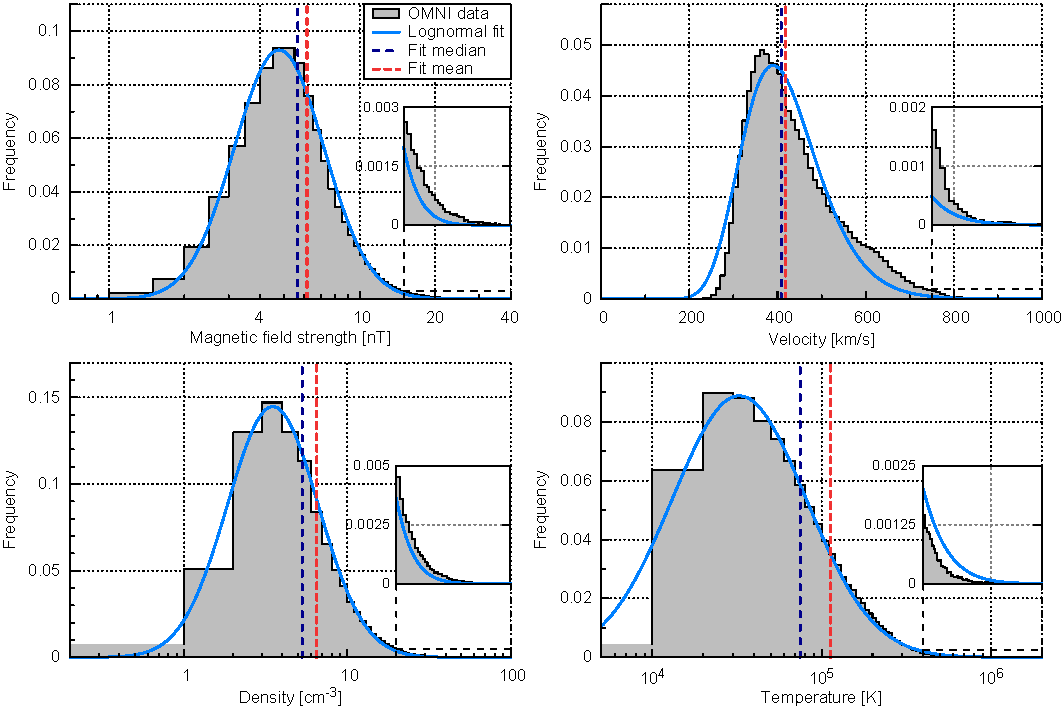
\includegraphics[width=18cm]{figures/histogram_fits_4_a_zoom_paper_pdfplot.pdf}
	\caption{Frequency distributions of the four solar wind parameters and their lognormal fits derived from the hourly OMNI data set. The histograms have bins of \SI{0.5}{\nT}, \SI{10}{\km\per\s}, \SI{1}{\per\cm\cubed} and \SI{10000}{\K}. The fits' median and mean values are indicated as well. The insets show zoomed-in \textbf{views of the high value tails of the distributions. } }
	\label{fig:histogram_fits_4_a_zoom_paper_pdfplot}
\end{figure*}

%double lognormal fitting
%%%%%%%%%%%%%%%%%%%%%%%%%
%justification for compositional lognormal fit
In order to find a better fit result for the velocity distribution, we assume that the velocity distribution can be made up of at least two overlapping branches \citep{McGregor2011b}. Therefore a compositional approach  is chosen by combining two lognormal functions (\ref{eq:single_lognormal_fit_function}), involving more fit variables:
\begin{align}
	W_\text{II}(x) &= c \cdot W_1(x) + (1 -c) \cdot W_2(x)\,.	\label{eq:double_lognormal_fit_function}
\end{align}
The balancing parameter $c$ ensures that the resulting function remains normalized as it represents a probability distribution.
The fitting of $W_\text{II}(x)$ to the velocity's frequency distribution yields the values of the now five fit parameters ($c$, $x_\text{med,1}$, $x_\text{avg,1}$, $x_\text{med,2}$ and $x_\text{avg,2}$) as listed in Table~\ref{tab:lognormal_fit_parameters} together with the median and mean values of the composed distribution, which can be derived via solving
\begin{align}
	\int W_\text{II}(x)\,\text{d}x = 0	&	&\text{and}	&	&\int x\,W_\text{II}(x)\,\text{d}x = 0	\,.
\end{align}
This more complex fit function is more accurate in describing the velocity's frequency distribution as shown in Fig.~\ref{fig:histogram_fits_V_a_zoom_dbl_paper_pdfplot}.
\begin{figure}
	\resizebox{\hsize}{!}{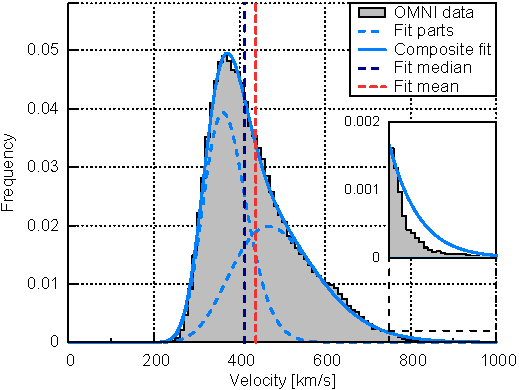
\includegraphics{figures/histogram_fits_V_a_zoom_dbl_paper_pdfplot.pdf}}
	\caption{\textbf{Velocity} frequency distribution (same as in Fig.~\ref{fig:histogram_fits_4_a_zoom_paper_pdfplot}) and its compositional lognormal fit. The fit's median and mean values and its two fit parts are indicated as well. \textbf{The inset is a zoomed-in view of the high value tail of the distribution. } }
	\label{fig:histogram_fits_V_a_zoom_dbl_paper_pdfplot}
\end{figure}
Thus in the following sections we keep the double lognormal ansatz for all velocity frequency fits.

%transition
For the bulk of the solar wind these static lognormal functions describe the parameters' distributions well\textbf{. The abnormally high parameter values in the distribution functions can be attributed to shock/CME events in agreement with the results of the OMNI solar wind investigations by \citet{Richardson2012}.} The simple lognormal fit functions underestimate the \textbf{frequencies in} their high value tails, except for the temperature’s tail which is overestimated, as seen in the insets of Fig.~\ref{fig:histogram_fits_4_a_zoom_paper_pdfplot}\textbf{, this appears to be because CMEs do not come with abnormally high temperatures, but rather with temperatures lower than those of the average solar wind \citep{Forsyth2006}.} The velocity's compositional lognormal fit only slightly overestimates its tail as seen in the inset of Fig.~\ref{fig:histogram_fits_V_a_zoom_dbl_paper_pdfplot}.
The slow and fast part contribute almost equally ($c \approx 0.5$) to the long-term velocity distribution function.

%{\color{red} discuss high value zoom figures; read in Veselovsky2010}


\section{Solar activity dependence of the solar wind frequency distributions}
\label{sec:solar_activity_variations}
In the next step we investigate how the long-term solar wind distribution functions presented in the previous section depend on general solar activity. Therefore we examine their correlation with the \textbf{SSN}, being a commonly used long-term solar activity index, and determine the time lags with the highest correlation coefficients.

%\subsection{SSN correlation}
For the correlations we fit lognormal functions to the frequency distributions as in Sect.~\ref{sec:frequency_distribution}, but implement linear relations to the yearly SSN, allowing shifting of the distribution functions with SSN. For the velocity the approach is different insofar as its two components are kept fixed and instead their balance is modified with the changing SSN. \textbf{Thus we obtain solar activity depending models for the frequency distributions of all four solar wind parameters.}

%\subsection{SSN data}
The international sunspot number (\citeyear{sidc}) is provided by the online catalogue\footnote{\url{http://www.sidc.be/silso/}} at the World Data Center -- Sunspot Index and Long-term Solar Observations (WDC-SILSO), Solar Influences Data Analysis Center (SIDC), Royal Observatory of Belgium (ROB).

Yearly medians of the solar wind parameters and the yearly SSN together with the solar cycle number \textbf{are shown in the upper part of Fig.~\ref{fig:OMNI_yearly_ssn_correlation_c_plot}}. The reason for correlating the SSN to the solar wind median values is because the position of a lognormal function is defined by its median. The data are averaged to yearly values to avoid seasonal effects during the Earth’s orbit around the Sun caused by its variations in solar latitude and distance.
\begin{figure}
	\resizebox{\hsize}{!}{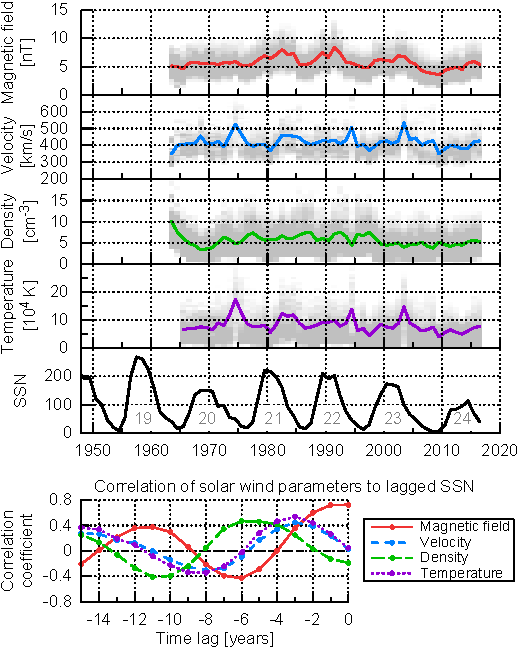
\includegraphics{figures/OMNI_yearly_ssn_correlation_c_plot.pdf}}
	\caption{\textbf{Solar} wind parameter yearly \textbf{frequencies (grey shading) with yearly medians (lines)} derived from OMNI data and the yearly SSN from the \citet{sidc} with solar cycle number (top). Their correlation coefficients with the yearly SSN are calculated for time lags back to -15 years (bottom).}
	\label{fig:OMNI_yearly_ssn_correlation_c_plot}
\end{figure}
The solar wind velocity, density and temperature depend on the state of the solar cycle \citep{Schwenn1983}. %density modulation with SSN \citep{Schwenn1983} p.~499\\
For instance the fast solar wind \textbf{occurs at times when polar coronal holes extend to lower latitudes, a typical feature of the declining phase of the solar cycle} as pointed out by \citet[p.~75, Figure~3.52]{Bothmer2007}. Therefore the solar wind velocity, density and temperature maxima exhibit \textbf{time lags relative} to the SSN maxima.

The correlation coefficients of the solar wind parameters with the yearly SSN shown in the bottom part of Fig.~\ref{fig:OMNI_yearly_ssn_correlation_c_plot} are calculated for time lags back to \num{-15}~years to cover a time span longer than a solar cycle. As expected, the \textbf{amplitudes of the variations in the correlations} of all parameters decline with increasing time lag and show a \textbf{period} of about 11~years. The highest correlation coefficient of 0.728 to the SSN is found for the magnetic field strength, it has no time lag. This finding is anticipated because the SSN is found to be directly proportional to the evolution of the photospheric magnetic flux \citep{Smith2003}.
Velocity and temperature show \textbf{time lags} of 3~years with peak correlation coefficients of 0.453 and 0.540. The density with a correlation coefficient of 0.468 has a time lag of 6~years, which is in agreement with the \textbf{density anticorrelation to the SSN} reported by \citet{Bougeret1984}.	%p.~406\\
% maximal correlation coefficients and their time lags:\\
% magnetic field strength: lag 0, 0.728\\
% velocity: lag -3, 0.453\\
% density: lag -6, 0.468\\
% temperature: lag -3, 0.540\\

%\subsection{SSN fitting}
\textbf{Next we create solar activity dependent analytical representations of the solar wind frequency distributions. This is achieved by shifting the median positions of the lognormal distributions as a linear function of the SSN. To enable these shifts}, we add a linear SSN dependency to the median
\begin{align}
	x_\text{med}(ssn) &= a_\text{med} \cdot ssn + b_\text{med}\,,	\label{eq:median_with_ssn}
\end{align}
using a factor to the SSN $a_\text{med}$ with a baseline $b_\text{med}$. We relate the mean with a scaling factor to the median to transfer its SSN dependency:
\begin{align}
	x_\text{avg}(ssn) &= \left(1 + a_\text{avg}\right) \cdot x_\text{med}(ssn)\,.	\label{eq:mean_with_ssn}
\end{align}
\textbf{These relations, substituted into the lognormal function (\ref{eq:single_lognormal_fit_function}), lead to a new SSN-dependent function $W'(x,ssn)$. This function} is then fitted to the yearly data\textbf{, using the yearly SSN as input parameter.} \textbf{The SSN is offset with the individual time lags determined before for each parameter, to benefit from the higher correlation. The values of} the three resulting fit coefficients ($a_\text{med}, b_\text{med}$ and $a_\text{avg}$) are presented in Table~\ref{tab:ssn_fit_parameters}.
\begin{table*}
	\caption{Resulting fit coefficients from the OMNI data\textbf{, based on the linear SSN dependencies (\ref{eq:median_with_ssn}) and (\ref{eq:mean_with_ssn})}. For the velocity the fit parameters from the double lognormal fit \textbf{(\ref{eq:double_lognormal_fit_function})} and their balancing function \textbf{(\ref{eq:balance_with_ssn})} are given. \textbf{The numbers in parentheses are the estimated standard deviations of the fit parameters referred to the corresponding last digits of the quoted value. The listed SSN time lags are used for the fits.}}
	\label{tab:ssn_fit_parameters}
	\centering
	\begin{tabular}{l@{} c@{}
		S[table-format = 1.3(2)e+1]
		S[table-format = 1.4(2)]
		S[table-format = 1.3(2)e+1]
		S[table-format = +1.3(2)e+1]
		c c
		}
		\hline\hline
		\multicolumn{2}{l}{\multirow{2}{*}{Parameter}}	&\multicolumn{2}{c}{Median}	&\multicolumn{1}{c}{Mean}	&\multicolumn{2}{c}{Balance}	&\multicolumn{1}{c}{SSN lag}\\
		\cline{3-4}\cline{6-7}
		\multicolumn{2}{l}{}	&\multicolumn{1}{c}{SSN factor $a_\text{med}$}	&\multicolumn{1}{c}{Baseline $b_\text{med}$}	&\multicolumn{1}{c}{Scaling factor $a_\text{avg}$}	&\multicolumn{1}{c}{SSN factor $c_a$}	&\multicolumn{1}{c}{Baseline $c_b$}	&\multicolumn{1}{c}{[years]}\\
		\hline
		\multicolumn{2}{l}{\textbf{Magnetic field [\si{nT}]}}	&1.309(19)e-2	&4.285(17)	&8.786(78)e-2	&\multicolumn{1}{c}{--}	&--	&0\\
%		\multicolumn{2}{l}{Velocity}	&2.514(93)e-3	&3.8521(90)	&2.392(26)e-2	&\multicolumn{1}{c}{--}	&--\\
		\multicolumn{2}{l}{\textbf{Density [\si{\per\cm\cubed}]}}	&3.81(25)e-3	&4.495(26)	&3.050(27)e-1	&\multicolumn{1}{c}{--}	&--	&6\\
		\multicolumn{2}{l}{\textbf{Temperature [\SI{e4}{\K}]}}	&1.974(26)e-2	&5.729(19)	&6.541(28)e-1	&\multicolumn{1}{c}{--}	&--	&3\\
		\hline
		\multicolumn{1}{l}{\textbf{Velocity}}	&\multicolumn{1}{c}{$W'_1$}	&\multicolumn{1}{c}{--}	&3.633(12)	&1.008(37)e-2	&\multirow{2}{*}{\tablenum{-1.799(95)e-3}}	&\multirow{2}{*}{0.638(32)}	&\multirow{2}{*}{3}\\
		\multicolumn{1}{l}{\textbf{[\SI{e2}{\km\per\s}]}}	&\multicolumn{1}{c}{$W'_2$}	&\multicolumn{1}{c}{--}	&4.831(81)	&2.31(20)e-2	&	&	&\\
		\hline
	\end{tabular}
\end{table*}

Naturally, the fit models match with the general data trends\textbf{, as can be seen from Fig.~\ref{fig:OMNI_yearly_BVdblNTSSN_fit_e_plot}}, though single year variations are not replicated by the model (e.g., the high velocity and temperature values in 1974, 1994 and 2003).
\begin{figure*}
	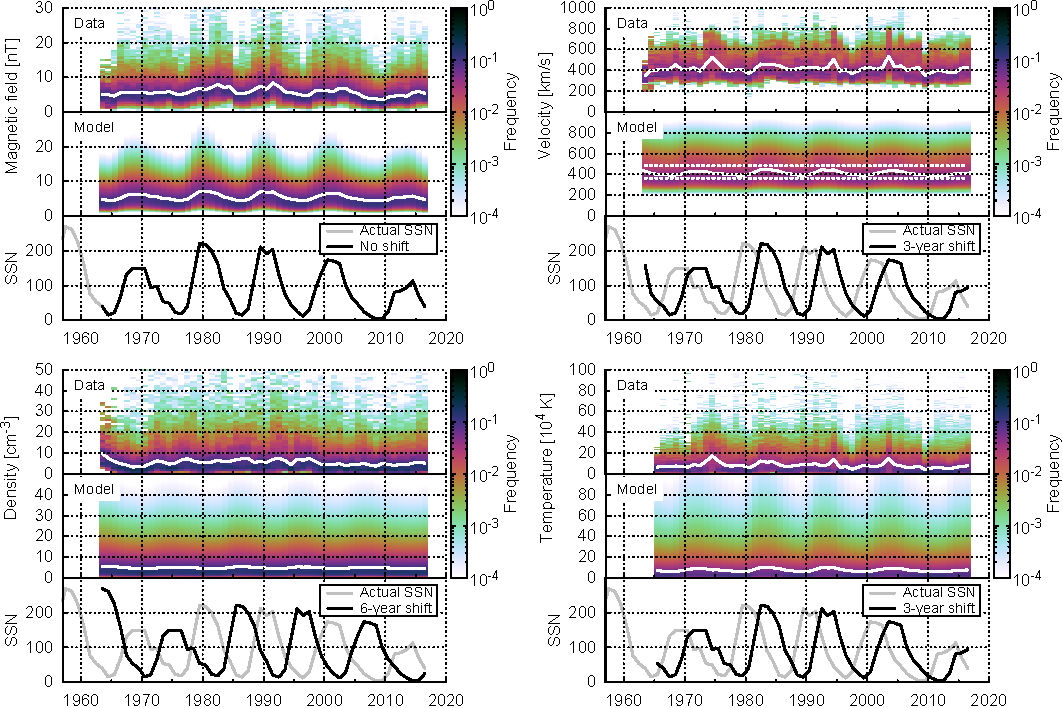
\includegraphics[width=18cm]{figures/OMNI_yearly_BVdblNTSSN_fit_e_plot.pdf}
	\caption{Solar wind parameter yearly data frequencies and lognormal fit models, both with their median values (white lines) over the OMNI time period 1963--2016. The corresponding yearly SSN and the \textbf{shifted SSN} for the models are indicated by grey and black lines. The velocity median is derived from the SSN-weighted constant lognormal parts (dotted lines).}
	\label{fig:OMNI_yearly_BVdblNTSSN_fit_e_plot}
\end{figure*}
The comparison of this model with the yearly data median values with respect to the lagged SSN shows that the medians obtained from the modeling have a quite similar slope, as shown in Fig.~\ref{fig:OMNI_yearly_BVNTvsSSN_a}.
\begin{figure}
	\resizebox{\hsize}{!}{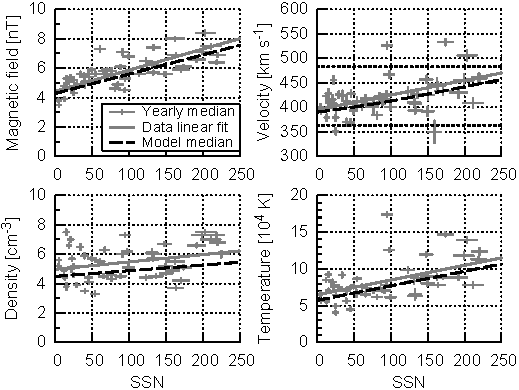
\includegraphics{figures/OMNI_yearly_BVNTvsSSN_a.pdf}}
	\caption{Solar wind parameter medians with respect to the lagged SSN. The yearly data medians (+) with their weighted linear fit (solid lines) are obtained from OMNI data. The error bars denote the SSN standard deviation and the relative weight from the yearly data coverage. The SSN-dependent median \textbf{(dashed lines)} is derived from the lognormal model fit. For the velocity the median is derived from the SSN-weighting (\ref{eq:balance_with_ssn}) of the slow and fast model parts \textbf{(dotted lines)}, whose magnitudes are SSN independent.}
	\label{fig:OMNI_yearly_BVNTvsSSN_a}
\end{figure}

Again, the solar wind velocity needs a special treatment because of the application of the double lognormal distribution (\ref{eq:double_lognormal_fit_function}). Since it is well known that slow and fast solar wind stream occurrence rates follow the solar cycle, we keep the two velocity components' positions \textbf{SSN-independent ($x_\text{med} =  b_\text{med}$)} and vary instead their balance with the SSN:
\begin{align}
	c(ssn) &= c_a \cdot ssn + c_b\,.	\label{eq:balance_with_ssn}
\end{align}
The fit result (see Table~\ref{tab:ssn_fit_parameters}) yields a model in which three years after solar cycle minimum (SSN of zero) the contribution of slow solar wind to the overall solar wind distribution reaches a maximum value \textbf{(about \SI{64}{\percent})} and decreases with increasing SSN as shown in Fig.~\ref{fig:Vdbl_SSN_ratio_f_plot}.
\begin{figure}
	\resizebox{\hsize}{!}{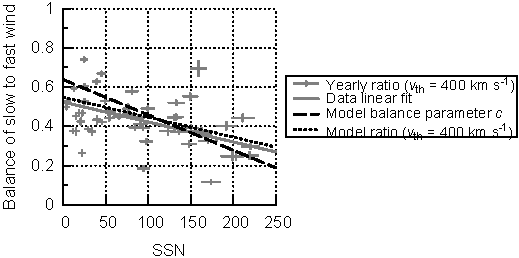
\includegraphics{figures/Vdbl_SSN_ratio_f_plot.pdf}}
	\caption{Ratio of slow to fast solar wind for a by 3~years lagged SSN. The yearly ratios (+) and their weighted linear fit (solid line) are obtained from OMNI data with a threshold velocity of $v_\text{th} = \SI{400}{\km\per\s}$. The error bars denote the SSN standard deviation and the relative weight from the yearly data coverage. The model's balance parameter (\ref{eq:balance_with_ssn}) and derived ratio (same threshold) are plotted as dashed and dotted lines.}
	\label{fig:Vdbl_SSN_ratio_f_plot}
\end{figure}
% 3 years after minimum (SSN of zero) the slow wind has its maximal share of 0.638(32). 3 years after maximum (SSN of 200) it has only a share of 0.278(37).

To investigate the amount of slow and fast wind contributions depending on solar activity, we apply the commonly used constant velocity threshold of $v_\text{th} = \SI{400}{\km\per\s}$ \citep[p.~144]{Schwenn1990}. The linear fit to the yearly data ratio and the derived model ratio show a good agreement (see Fig.~\ref{fig:Vdbl_SSN_ratio_f_plot}). \textbf{The to some degree steeper balance parameter of the double fit function used in this model cannot be compared directly with} specific velocity thresholds between slow and fast solar wind. However, it appears being likely a more realistic approach than just taking a specific velocity threshold for the slow and fast wind, in agreement with the overlapping nature of the velocity flows reported by \citet{McGregor2011b}.
%(i.e. there exists slow wind with properties of fast wind and vice versa)


%exponential fitting
%%%%%%%%%%%%%%%%%%%%
\section{Solar distance dependency}
\label{sec:solar_distance_dependency}
In order to derive heliocentric distance relationships of the bulk solar wind distribution functions, we apply and fit \textbf{power law dependencies} to the Helios data. We evaluate the fits’ extrapolation behavior in direction to the Sun, because in a subsequent step \textbf{they are} extrapolated to the PSP orbit. We use the fitting methods of Sect.~\ref{sec:frequency_distribution} for the distance-binned combined data from both Helios probes. Helios’ highly elliptical orbits in the ecliptic covered a solar distance range of \SIrange{0.31}{0.98}{\au} in case of Helios~1 and \SIrange{0.29}{0.98}{\au} in case of Helios~2. Launched during solar cycle minimum, the data of both probes cover the rise to the maximum of cycle~21, covering $\sim$6.5~years at varying distances to the Sun.

We investigate hourly averages of the Helios data \textbf{in the same way as with the OMNI data}. The Helios~1 merged hourly data from the magnetometer and plasma instruments \citep{Rosenbauer1977} include $\sim$12.5~orbits for the time range 10~December 1974 until 14~June 1981, those for Helios~2 include $\sim$8~orbits for the time span 1~January 1976 until 4~March 1980. The data are retrieved from the Coordinated~Data~Analysis~Web (CDAWeb) interface at NASA's GSFC/SPDF\footnote{\url{http://spdf.gsfc.nasa.gov/}}.
%Helios plasma instrument (E1); Helios magnetometer instrument (E2)
% Helios data ranges:\\
% - time range Helios~1 [1974-12-10--1981-06-14] (12.5~orbits), Helios~2 [1976-01-01--1980-03-04] (8~orbits)\\
% - solar distance range Helios~1 0.31--0.98~au, Helios~2 0.29--0.98~au\\
%data sources

The Helios~1 magnetometer data coverage for this data set is about \SI{43}{\%} (i.e., 2.8~years), that of Helios~2 amounts to \SI{54}{\%} (i.e., 2.3~years). The plasma data coverage is \SI{76}{\%} (i.e., 5.0~years) in case of Helios~1 and \SI{92}{\%} (i.e., 3.9~years) in case of Helios~2. 
% temporal coverage of merged data\\
% Helios 1: 1974-12-10--1981-06-14; 6y6m15d = 2388~d = 6.538~y\\
% Mag data coverage: 42.6~\%; 2.785~years\\
% Plasma data coverage: 76.4~\%; 4.995~years\\
% Helios 2: 1976-01-01--1980-03-04; 4y3m4d = 1557~d = 4.263~y\\
% Mag data coverage: 54.4~\%; 2.319~years (83~\% of H1)\\
% Plasma data coverage: 91.8~\%; 3.913~years (78~\% of H1)\\
%Helios data biased towards solar minimum
Thus, using this data, \textbf{we point out} that its time coverage is unequally distributed over the solar cycle. Considering the data gap distributions, the amount of data during solar cycle minimum up to mid~1977, that is, the transition from minimum to maximum, covers about \SI{68}{\percent} \textbf{of this period} whereas during maximum of cycle~21 data are available only \SI{38}{\percent} of the time. This Helios data bias towards solar minimum is \textbf{one} reason why in this study the Helios solar wind data are not used to derive long-term frequency distributions and solar cycle dependencies for the key solar wind parameters.
% data gaps -> uneven coverage -> solar cycle minimum dominates; ratio of max vs min cycle data coverage; for OMNI data negligible\\
% 13~months smoothed sunspot number \citep{sidc}: divide June~1977 (include figure)\\
% put link on sidc webpage: http://sidc.be/sunspot-data/SIDCpub.php
% begin: 1974-12 36.1\\
% minimum: May/June 1976 18.3/17.9 (cite?)\\
% divide 30~June~1977 37.7 from SIDC data (nearly same SSN as at Helios~1 beginning)\\
% cycle 21 maximum: Dec 1979 232.9 (cite?)\\
% end: 1981-06 200.9\\
% 
% data gap hours and percentages:\\
% % H1 minimum 22416 h\\
% % H1 maximum 34681 h\\
% % H2 minimum 13128 h\\
% % H2 maximum 23472 h\\
% % sum 93697 h\\
% solar minimum: 35\,544~h, 37.94~\%\\
% solar maximum: 58\,153~h, 62.06~\%\\

% 1974 11 1974.874   39.3   4.2    30  
% 1974 12 1974.958   36.1   4.0    31  
% 1975 01 1975.042   33.0   3.9    31  
% 1975 02 1975.123   31.8   3.8    28  
% 1975 03 1975.204   30.6   3.7    31  
% 1975 04 1975.288   26.8   3.5    30  
% 1975 05 1975.371   24.2   3.3    31  
% 1975 06 1975.455   23.2   3.3    30  
% 1975 07 1975.538   21.8   3.2    31  
% 1975 08 1975.623   20.7   3.1    31  
% 1975 09 1975.707   20.9   3.1    30  
% 1975 10 1975.790   22.3   3.2    31  
% 1975 11 1975.874   23.3   3.3    30  
% 1975 12 1975.958   23.6   3.3    31  
% 1976 01 1976.042   22.1   3.2    31  
% 1976 02 1976.124   19.2   3.0    29  
% 1976 03 1976.206   17.8   2.9    31  
% 1976 04 1976.290   18.4   2.9    30  
% 1976 05 1976.373   18.3   2.9    31  
% 1976 06 1976.456   17.9   2.9    30  
% 1976 07 1976.540   18.8   2.9    31  
% 1976 08 1976.624   20.5   3.1    31  
% 1976 09 1976.708   20.8   3.1    30  
% 1976 10 1976.791   19.7   3.0    31  
% 1976 11 1976.874   19.7   3.0    30  
% 1976 12 1976.958   21.6   3.2    31  
% 1977 01 1977.042   24.3   3.3    31  
% 1977 02 1977.123   26.3   3.5    28  
% 1977 03 1977.204   28.8   3.6    31  
% 1977 04 1977.288   31.9   3.8    30  
% 1977 05 1977.371   34.7   4.0    31  
% 1977 06 1977.455   37.7   4.1    30  
% 1977 07 1977.538   41.4   4.3    31  
% 1977 08 1977.623   47.6   4.6    31  
% 1977 09 1977.707   55.8   5.0    30  
% 1977 10 1977.790   64.8   5.4    31  
% 1977 11 1977.874   73.7   5.7    30  
% 1977 12 1977.958   80.7   6.0    31  
% 1978 01 1978.042   86.9   6.2    31  
% 1978 02 1978.123   91.5   6.4    28  
% 1978 03 1978.204   98.7   6.6    31  
% 1978 04 1978.288  109.0   7.0    30  
% 1978 05 1978.371  117.8   7.2    31  
% 1978 06 1978.455  126.6   7.5    30  
% 1978 07 1978.538  138.0   7.8    31  
% 1978 08 1978.623  147.3   8.1    31  
% 1978 09 1978.707  153.6   8.3    30  
% 1978 10 1978.790  157.3   8.4    31  
% 1978 11 1978.874  160.4   8.5    30  
% 1978 12 1978.958  166.7   8.6    31  
% 1979 01 1979.042  175.2   8.8    31  
% 1979 02 1979.123  185.4   9.1    28  
% 1979 03 1979.204  193.3   9.3    31  
% 1979 04 1979.288  199.9   9.4    30  
% 1979 05 1979.371  208.5   9.6    31  
% 1979 06 1979.455  216.7   9.8    30  
% 1979 07 1979.538  219.5   9.9    31  
% 1979 08 1979.623  220.1   9.9    31  
% 1979 09 1979.707  220.4   9.9    30  
% 1979 10 1979.790  223.4  10.0    31  
% 1979 11 1979.874  229.8  10.1    30  
% 1979 12 1979.958  232.9  10.2    31  
% 1980 01 1980.042  232.0  10.2    31  
% 1980 02 1980.124  230.2  10.2    29  
% 1980 03 1980.206  227.9  10.1    31  
% 1980 04 1980.290  224.6  10.0    30  
% 1980 05 1980.373  221.3  10.0    31  
% 1980 06 1980.456  219.1   9.9    30  
% 1980 07 1980.540  216.1   9.9    31  
% 1980 08 1980.624  212.0  10.0    31  
% 1980 09 1980.708  211.5  10.2    30  
% 1980 10 1980.791  211.9  10.5    31  
% 1980 11 1980.874  209.1  10.9    30  
% 1980 12 1980.958  202.8  11.0    31  
% 1981 01 1981.042  199.6  11.1   271  
% 1981 02 1981.123  202.2  11.5   229  
% 1981 03 1981.204  205.4  12.1   244  
% 1981 04 1981.288  205.7  12.6   254  
% 1981 05 1981.371  204.1  12.8   268  
% 1981 06 1981.455  200.9  13.1   227  
% 1981 07 1981.538  198.5  13.1   268  

\textbf{The radial dependencies of the key solar wind parameters over the distance range \SIrange{0.29}{0.98}{\au} measured by both Helios probes are plotted in Fig.~\ref{fig:radial_fit_4_thesis_light_b_skip}, together with their median and mean values for different solar distances, calculated for the minimal distance resolution \SI{0.01}{\au} of the data set.}
\begin{figure*}
	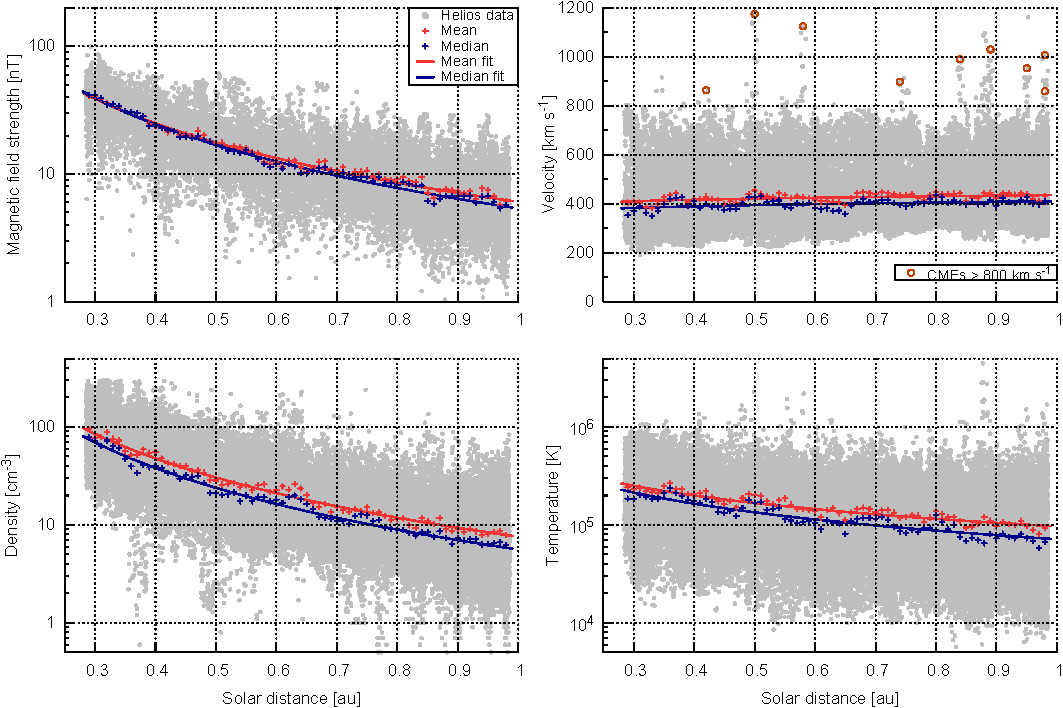
\includegraphics[width=18cm]{figures/radial_fit_4_thesis_light_b_skip.pdf}
	\caption{Helios hourly data plots of the four solar wind parameters over solar distance. The mean and median per \SI{0.01}{\au} data bin and their fit curves are plotted as well. The Helios data has a native distance resolution of \SI{0.01}{\au}, thus, to make the abundance visible in these plots, we added a random distance value of up to \SI{+-0.005}{\au}. \textbf{The high velocity data points above \SI{800}{\km\per\s} (circled red) are identified as CME events \citep[e.g.,][]{Sheeley1985,Bothmer1996,Bothmer1998}.}}
	\label{fig:radial_fit_4_thesis_light_b_skip}
\end{figure*}
Assuming a radial solar wind outflow, it is expected that the distance dependence of the solar wind parameters over the Helios data range \SIrange{0.29}{0.98}{\au} can be described through power law scaling. Therefore we use the power law function
\begin{align}
	x(r) = d\cdot r^e	\label{eq:power_function}
\end{align}
for the regression fit of the median and mean, with $r$ being the solar distance in astronomical units, $d$ the magnitude at \SI{1}{\au} and $e$ the exponent. The fits are weighted through the different data counts per bin.
%fit result table and figure
\textbf{The obtained coefficients for the median and mean power law fits ($d_\text{med}$, $e_\text{med}$, $d_\text{avg}$ and $e_\text{avg}$) are listed in Table~\ref{tab:mean_median_fit_parameter} and their corresponding curves are shown in Fig.~\ref{fig:radial_fit_4_thesis_light_b_skip}.}
\begin{table*}
	\caption{Fit coefficients for the median and mean solar distance dependencies \textbf{(\ref{eq:power_function})} of the four solar wind parameters derived from the combined Helios~1 and 2 data. \textbf{The numbers in parentheses are the estimated standard deviations of the fit parameters referred to the corresponding last digits of the quoted value.} The crossing distances indicate where the median and mean fits intersect each other. The yearly variation is the weighted standard deviation derived from the yearly fit exponents seen in Fig.~\ref{fig:yearly_gradients_c}.}
	\label{tab:mean_median_fit_parameter}
	\centering
	\begin{tabular}{l
	S[table-format = 1.3(2)]
	S[table-format = +1.3(2)]
	@{}c
	S[table-format = 1.3(2)]
	S[table-format = +1.3(2)]
	S[table-format = 1.1(2)e1]
	S[table-format = 1.3]}
		\hline\hline
		\multirow{2}{*}{Parameter}	&\multicolumn{2}{c}{Median}	&	&\multicolumn{2}{c}{Mean}	&\multicolumn{1}{c}{Crossing distance}	&\multicolumn{1}{c}{Yearly variation}\\
		\cline{2-3}	\cline{5-6}
			&\multicolumn{1}{c}{$d_\text{med}$}	&\multicolumn{1}{c}{$e_\text{med}$}	&	&\multicolumn{1}{c}{$d_\text{avg}$}	&\multicolumn{1}{c}{$e_\text{avg}$}	&\multicolumn{1}{c}{[\si{\au}]}	&\multicolumn{1}{c}{$\Delta e$}\\
		\hline
		\textbf{Magnetic field [\si{nT}]}	&5.377(92)	&-1.655(17)	&	&6.05(10)	&-1.546(18)	&0.339(11)	&0.11\\
		\textbf{Velocity [\SI{e2}{\km\per\s}]}	&4.107(28)	&0.058(13)	&	&4.356(24)	&0.049(10)	&0.7(83)e3	&0.012\\
		\textbf{Density [\si{\per\cm\cubed}]}	&5.61(27)	&-2.093(46)	&	&7.57(30)	&-2.010(38)	&0.027(73)	&0.072\\
		\textbf{Temperature [\SI{e4}{\K}]}	&7.14(23)	&-0.913(39)	&	&9.67(21)	&-0.792(28)	&0.082(85)	&0.050\\
		\hline
	\end{tabular}
\end{table*}
% source year variation: fit_out_yearly_gradients_table_b_stats.txt

% comparison with other Helios studies (Schwenn, Bougeret)
%Helios results, radial gradients see \citet{Schwenn1990} p.~155
\textbf{Our derived} exponents agree with those found in existing studies from the Helios observations: \citet{Mariani1978} derived the exponents for the magnetic field strength separately for the fast and slow solar wind as $B_\text{fast} \propto r^{-1.54}$ and $B_\text{slow} \propto r^{-1.61}$\textbf{, ours is $B_\text{avg} \propto r^{-1.55}$}.
%$B_\text{fast} = 5.79\cdot r^{-1.54}$\,nT and $B_\text{slow} = 5.11\cdot r^{-1.61}$\,nT.
The velocity exponent \textbf{$v_\text{avg} \propto r^{0.049}$} matches with the values found by \citet{Schwenn1983,Schwenn1990}, who derived the distance dependencies for both Helios spacecraft separately as $v_\text{H1} \propto r^{0.083}$ and $v_\text{H2} \propto r^{0.036}$. The calculated density exponent \textbf{$n_\text{avg} \propto r^{-2.01}$} agrees well with the Helios plasma density model derived by \citet{Bougeret1984} yielding $n \propto r^{-2.10}$.
%to the year 1976 normalized   a \SI{1}{\au} density of $n = 6.14\cdot r^{-2.10}\,\text{cm}^{-3}$.
The temperature exponent \textbf{$T_\text{avg} \propto r^{-0.79}$} is similar to those in the studies by \citet{Hellinger2011,Hellinger2013}, who also derived the exponents separately for the fast and the slow solar wind: $T_\text{fast} \propto r^{-0.74}$ and $T_\text{slow} \propto r^{-0.58}$.
%$T_\text{fast} = \num{2.5e5} (R/R_0)^{-0.74}$\,K and $T_\text{slow} = \num{6.2e4} (R/R_0)^{-0.58}$\,K.
%\citet{Marsch1982}	$T_\text{||,slow} \propto r^{-1.03}$ and $T_\text{||,fast} \propto r^{-0.69}$.

%crossing distances
\textbf{The mean and median velocity fit exponents acquired from the Helios data} are very similar, which indicates that they just as well can be kept identical so that the basic shape of the frequency distribution does not change with distance. Contrary, the mean and median fits for the magnetic field strength cross each other at \SI{0.339}{\au} \textbf{(see Table~\ref{tab:mean_median_fit_parameter})} and the mean is \textbf{getting slightly} lower than the median at smaller distances. Thus, below that distance the \textbf{frequency distribution} cannot well be described anymore by a lognormal function\textbf{, because the mean of a lognormal function has to be larger than its median (as pointed out in Sect.~\ref{sec:frequency_distribution}), that is, the location of the crossing indicates that the parameter's distribution is not anymore of a lognormal shape thereafter.} The fits for the proton temperature show a similar behavior, having an \textbf{extrapolated} intersection at \SI{0.082}{\au}. Therefore the extrapolation of the magnetic field and temperature distribution frequencies to the PSP orbit by applying lognormal functions is limited. \textbf{The crossing points limit the regions where the distribution's shapes can still be considered lognormal.}

\textbf{In order to still fit and extrapolate lognormal functions with the data, we assume that the shapes can be considered lognormal at all distances. For the coming frequency distribution fit function we reduce the fit exponents $e_\text{med}$ and $e_\text{avg}$ to only one. We note} that this simplification leads to slightly larger modeling errors, especially in case of the magnetic field strength.

%\subsection{Power law lognormal fitting}
Next we retrieve the frequency distributions of the four \textbf{solar wind parameters in solar} distance bins of \SI{0.01}{\au}, choosing the same resolution as for the OMNI data analyzed in Sect.~\ref{sec:frequency_distribution} -- the distributions \textbf{and their median values} are plotted in Fig.~\ref{fig:mixed_fit_fixed_4_paper_f_plot}.
\begin{figure*}
	\includegraphics[width=18cm]{figures/mixed_fit_fixed_4_paper_f_plot.pdf}
	\caption{Frequency distributions of the four solar wind parameters with respect to solar distance. Plotted are the binned Helios data and the power law lognormal fit models with their median values (white lines). The double lognormal model is used for the velocity, its slow and fast parts are indicated by dotted lines.}
	\label{fig:mixed_fit_fixed_4_paper_f_plot}
\end{figure*}
% Helios histogram bin sizes for mean of frequency distribution (at specific solar distance):\\
% $B$: bin size 0.5~nT, min 337, mean precision: 0.000545\\
% $v$: bin size 1~cm$^{-3}$, min 497, mean precision: 0.00449\\
% $n$: bin size 10~km/s, min 497, mean precision:  0.00449\\
% $T$: bin size 10\,000~K, min 497, mean precision: 4.49--44.49\\
For simplification, as mentioned before, we treat the exponents of the median and mean fit functions as being identical\textbf{, using one fit parameter for both.} Implementing the power law distance dependency~(\ref{eq:power_function}) into the lognormal function (\ref{eq:single_lognormal_fit_function}), we get the fit parameters $d'_\text{med}$, $d'_\text{avg}$ and \textbf{the} common exponent $e'$. Again, we use the double lognormal function~(\ref{eq:double_lognormal_fit_function}) for the velocity distribution fit -- resulting in $W''_\text{II}(x,r)$. The additional fit parameters are the balancing parameter $c'$ and for the second lognormal part $d'_\text{med,2}$ and $d'_\text{avg,2}$. The resulting fit coefficients for the four solar wind parameters are presented in Table~\ref{tab:extrapolation_model_fit_parameters}.
\begin{table*}
	\caption{Fit coefficients \textbf{for the distance depending single lognormal function, based on equation (\ref{eq:single_lognormal_fit_function}) combined with (\ref{eq:power_function})}, respectively double lognormal \textbf{function (\ref{eq:double_lognormal_fit_function})} for the velocity from the combined Helios data. \textbf{The numbers in parentheses are the estimated standard deviations of the fit parameters referred to the corresponding last digits of the quoted value.} The seasonal variations are calculated from Earth's orbital solar distance variation and the derived exponents.}
	\label{tab:extrapolation_model_fit_parameters}
	\centering
	\sisetup{table-figures-integer=1, table-figures-decimal=3, table-figures-exponent=0}
	\begin{tabular}{l c
	S[table-format = 1.3(2), table-space-text-post = a, table-align-text-post = false]
	S[table-format = 1.3(2), table-space-text-post = a, table-align-text-post = false]
	S[table-format = +1.4(2)]
	S[table-format = 1.3(2)]
	S[table-format = 1.2]}
		\hline\hline
		\multicolumn{2}{l}{\multirow{2}{*}{Parameter}}	&\multicolumn{1}{c}{Median}	&\multicolumn{1}{c}{Mean}	&\multicolumn{1}{c}{Exponent}	&\multicolumn{1}{c}{Balance}	&\multicolumn{1}{c}{Seasonal variation}\\
			&	&\multicolumn{1}{c}{$d'_\text{med}$}	&\multicolumn{1}{c}{$d'_\text{avg}$}	&\multicolumn{1}{c}{$e'$}	&$c'$	&\multicolumn{1}{c}{$\Delta d$ [\%]}\\
		\hline
		\multicolumn{2}{l}{\textbf{Magnetic field [\si{nT}]}}	&5.358(25)	&5.705(28)	&-1.662(11)	&\multicolumn{1}{c}{--}	&2.8\\
		\multicolumn{2}{l}{\textbf{Density [\si{\per\cm\cubed}]}}	&5.424(33)	&6.845(47)	&-2.114(20)	&\multicolumn{1}{c}{--}	&3.6\\
		\multicolumn{2}{l}{\textbf{Temperature [\SI{e4}{\K}]}}	&6.357(64)	&10.72(14)	&-1.100(20)	&\multicolumn{1}{c}{--}	&1.9\\
		\hline
		\multirow{2}{*}{\textbf{Velocity}}	&$W''_1$	&3.707(13)	&3.748(16)	&\multirow{2}{*}{0.0990(51)}	&\multirow{2}{*}{0.557(45)}	&\multicolumn{1}{c}{\multirow{2}{*}{0.17}}\\
		\multirow{2}{*}{\textbf{[\SI{e2}{\km\per\s}]}}	&$W''_2$	&5.26(13)	&5.42(11)	&	&	&\\
		\cline{2-7}
			&$W''_\text{II}$	&4.13(13)\tablefootmark{a}	&4.47(11)\tablefootmark{a}	&\multicolumn{1}{c}{--}	&\multicolumn{1}{c}{--}	&\multicolumn{1}{c}{--}\\
		\hline
	\end{tabular}
	\tablefoot{
		\tablefoottext{a}{Velocity median and mean \SI{1}{\au} values for the resulting function. Error estimates derived from the individual fit part errors.}
	}
\end{table*}
% Vdbl fit:
% medians = 370.7, 526
% means = 374.8, 542
% c = 0.557
% via calculate_twolognormal_median.py:
% mean = 446.64
% median = 413.33
%
% Yearly Earth distance variations from Earth_orbit_variation_impact_estimate.ods

The velocity balancing parameter $c' = 0.557$ is in good agreement with the results for the SSN dependency (\ref{eq:balance_with_ssn}), because with a mean SSN of 59 during the Helios time period, $c(59) = 0.53$, as can be seen from Fig.~\ref{fig:Vdbl_SSN_ratio_f_plot}.

\textbf{The power law lognormal models and the power law double lognormal model for the velocity, which result from the fitting, are plotted in Fig.~\ref{fig:mixed_fit_fixed_4_paper_f_plot} together with their median values.} The model’s magnetic field strength is broader around values of \SI{40}{nT} at the lower distance boundary than the data's frequency distribution implies. This behavior is expected because of the distance independent shape approximation applied. The velocity and temperature models’ upper values generally show a higher abundance than the actual data, see also zoom boxes in Figs.~\ref{fig:histogram_fits_4_a_zoom_paper_pdfplot} and \ref{fig:histogram_fits_V_a_zoom_dbl_paper_pdfplot}. \textbf{The with distance increasing high velocity tail arises} from using the same exponent for both slow and fast components. This effect is not seen in the data, more specifically, not only the slowest wind but also the fastest wind is expected to converge to more average speeds \citep{Sanchez-Diaz2016}.
%\citep{Sanchez-Diaz2016} p.~2835, using MHD-model -> very slow solar wind is continuation of slow wind) (because of interaction)


\section{Empirical solar wind model}
\label{sec:empirical_solar_wind_model}
In order to estimate the solar wind environment for the PSP orbit, we combine the results from the solar wind frequency distributions’ solar activity relationships and their distance dependencies derived from the OMNI and Helios data. The result is an empirical solar wind model for the inner heliosphere which \textbf{is then} extrapolated to the PSP orbit in Sect.~\ref{sec:model_extrapolation_to_psp_orbit}.

%\subsection{Distance scaling law variations}
%\label{sec:distance_scaling_law_variations}
\textbf{This solar wind model} for the radial distance dependence is representative for the time of the Helios observations around the rise of solar cycle~21. The \textbf{variations of the} yearly power law fit exponents \textbf{from fitting the solar distance dependency (\ref{eq:power_function})} are shown in Fig.~\ref{fig:yearly_gradients_c} together with the yearly SSN for the time period \numrange{1974}{1982}. It can be seen that during the Helios time period there might be some systematic  variation of the exponents with solar activity -- at least for the velocity and temperature exponents.
\begin{figure}
	\resizebox{\hsize}{!}{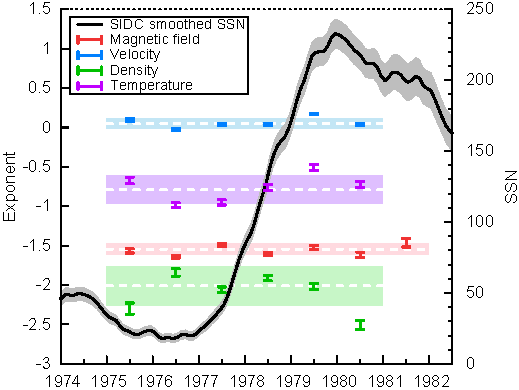
\includegraphics{figures/yearly_gradients_c.pdf}}
	\caption{Helios yearly variation of the solar wind \textbf{parameter power exponents for the dependence on radial distance} together with the SIDC 13-month smoothed monthly SSN. The weighted standard deviations and average values for all years are indicated by the shaded areas. In this plot the 21~days since Helios launch in the year 1974 are omitted because a distance range of merely \SIrange{0.95}{0.98}{\au} was covered that year.}
	\label{fig:yearly_gradients_c}
\end{figure}
%yearly variation of the solar wind parameters' average fit function exponents
However, for simplicity we assume that the distance scaling laws can be treated as time independent and include the calculated exponents’ yearly variations $\Delta e$, summarized in Table~\ref{tab:mean_median_fit_parameter}, as relative uncertainties.

Since we neglect possible variations of the distance scaling laws, we combine the frequency distribution’s median solar activity dependency (\ref{eq:median_with_ssn}) derived for \SI{1}{\au} from the OMNI data with the power law exponents (\ref{eq:power_function}) derived from the Helios data:
\begin{align}
	x_\text{med}(ssn,r) &= \left(a_\text{med} \cdot ssn + b_\text{med}\right) \cdot r^{e'}	\,.	\label{eq:general_sw_model}
\end{align}
Thus\textbf{, implementing the median and mean relations into the lognormal function (\ref{eq:single_lognormal_fit_function}),} we obtain the combined model function $W'''(x,ssn,r)$ and for the velocity $W_\text{II}'''(x,ssn,r)$ with the double lognormal function (\ref{eq:double_lognormal_fit_function}). \textbf{The corresponding median and mean relations for each solar wind parameter, based on the values resulting from our analyses, are listed below. Their numerical values are the fit parameters from Table~\ref{tab:ssn_fit_parameters} and the exponents from Table~\ref{tab:extrapolation_model_fit_parameters}.}

\textbf{\begin{itemize}
	\item The magnetic field strength relations, depending on solar activity and solar distance, are:
	\begin{align}
		B_\text{med}(ssn,r) &= \left(\SI{0.0131}{\nT} \cdot ssn + \SI{4.29}{\nT}\right) \cdot r^{-1.66}	\,,	\label{eq:median_B}\\
		B_\text{avg}(ssn,r) &= 1.0879 \cdot B_\text{med}(ssn,r)\,.
	\end{align}
	\item The proton velocity relations for the slow and fast components, depending on solar distance, are:
	\begin{align}
		v_\text{med}^\text{slow}(r) &= \SI{363}{\km\per\s} \cdot r^{0.099}	\,,&	&	&v_\text{med}^\text{fast}(r) &= \SI{483}{\km\per\s} \cdot r^{0.099}	\,,	\label{eq:median_v}\\
		v_\text{avg}^\text{slow}(r) &= 1.0101 \cdot v_\text{med}^\text{slow}(r)	\,,&	&	&v_\text{avg}^\text{fast}(r) &= 1.023 \cdot v_\text{med}^\text{fast}(r)	\,.
	\end{align}
	The share of both components balanced with solar activity is found to be:
	\begin{align}
		c(ssn) = -0.00180 \cdot ssn + 0.64	\,.	\label{eq:balance_v}
	\end{align}
	\item The derived relations of the proton density are:
	\begin{align}
		n_\text{med}(ssn,r) &= \left(\SI{0.0038}{\per\cm\cubed} \cdot ssn + \SI{4.50}{\per\cm\cubed}\right) \cdot r^{-2.11}	\,,	\label{eq:median_n}\\
		n_\text{avg}(ssn,r) &= 1.305 \cdot n_\text{med}(ssn,r)\,.
	\end{align}
	\item The derived proton temperature relations are:
	\begin{align}
		T_\text{med}(ssn,r) &= (\SI{197}{\K} \cdot ssn + \SI{57300}{\K}) \cdot r^{-1.10}	\,,	\label{eq:median_T}\\
		T_\text{avg}(ssn,r) &= 1.654 \cdot T_\text{med}(ssn,r)\,.
	\end{align}
\end{itemize}}

\textbf{These relations average} over seasonal variations because \textbf{they are} based on yearly data. \textbf{The} OMNI data are time-shifted to the nose of the Earth’s bow shock, this leads to yearly solar distance variations of \SI{+-1.67}{\%} as it orbits the Sun. The resulting maximal solar wind parameter variation amplitudes over the year can thus be derived from the derived power law exponents. They are estimated to be smaller than \SI{4}{\percent} as seen in Tab.~\ref{tab:extrapolation_model_fit_parameters}. \citet{Bruno1986} \textbf{and} \citet{Balogh1999} have pointed out, that the solar wind parameters vary with latitudinal separation from the heliospheric current sheet. Its position in heliographic latitude is highly variable around the solar equator \citep{Schwenn1990}, furthermore, the Earth’s orbit varies over the course of the year by \SI{+-7.2}{\degree} in latitude. \textbf{Since this latitudinal separation is highly variable and requires significant effort to calculate for an extended time series, we have ignored this aspect in this analysis.}	%Balogh et al. (p.~162, 1999);	 (Schwenn 1990, p.~126)


\section{Model extrapolation to PSP orbit}
\label{sec:model_extrapolation_to_psp_orbit}
To estimate PSP’s solar wind environment during its mission time for its orbital positions, \textbf{predictions of the SSN during the mission are incorporated into the empirical solar wind model, derived in the previous sections,} and extrapolations down to the PSP perihelion region are performed.

%\subsection{Near-Sun extrapolation for PSP orbit}
%PSP orbit
Parker Solar Probe is planned to launch in mid 2018. With its first Venus flyby it will swing into Venus' orbital plane, reaching already 93~days after launch in November 2018 a first perihelion with a distance of \SI{0.16}{\au}. Seven additional Venus flybys allow \textbf{the perihelion distance to be reduced} to a minimum of \SI{9.86}{\Rs}\textbf{. This distance will be reached with the 22nd perihelion in December 2024 \citep{Fox2015}, as plotted in the top panel of Fig.~\ref{fig:SPP_orbit_predicted_SSN_overview_f_plot}}.
\begin{figure}
	\resizebox{\hsize}{!}{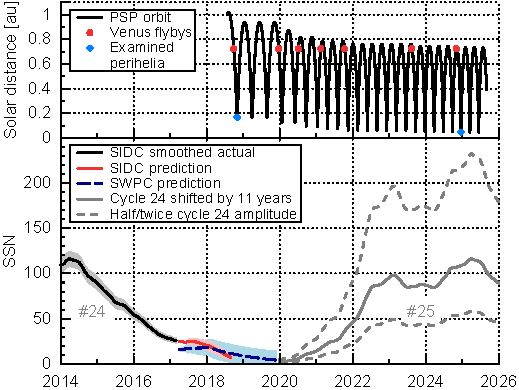
\includegraphics{figures/SPP_orbit_predicted_SSN_overview_f_plot.pdf}}
	\caption{PSP's solar distance during its mission time (top). Consecutive Venus flybys bring its perihelia nearer to the Sun. Actual and predicted SSN (bottom), that is, SIDC 13-month smoothed monthly actual SSN, SIDC \textbf{Standard Curves Kalman filter} prediction, SWPC prediction and by 11~years shifted SSN from previous cycle~24, together with two alternative trends of half and twice its amplitude.}
	\label{fig:SPP_orbit_predicted_SSN_overview_f_plot}
\end{figure}

We extrapolate the derived empirical solar wind \textbf{models} to PSP’s orbital distance range and compare the results with those from the existing models shown in Fig.~\ref{fig:sw_extrapolation_ssn_f_plot}.
\begin{figure*}
	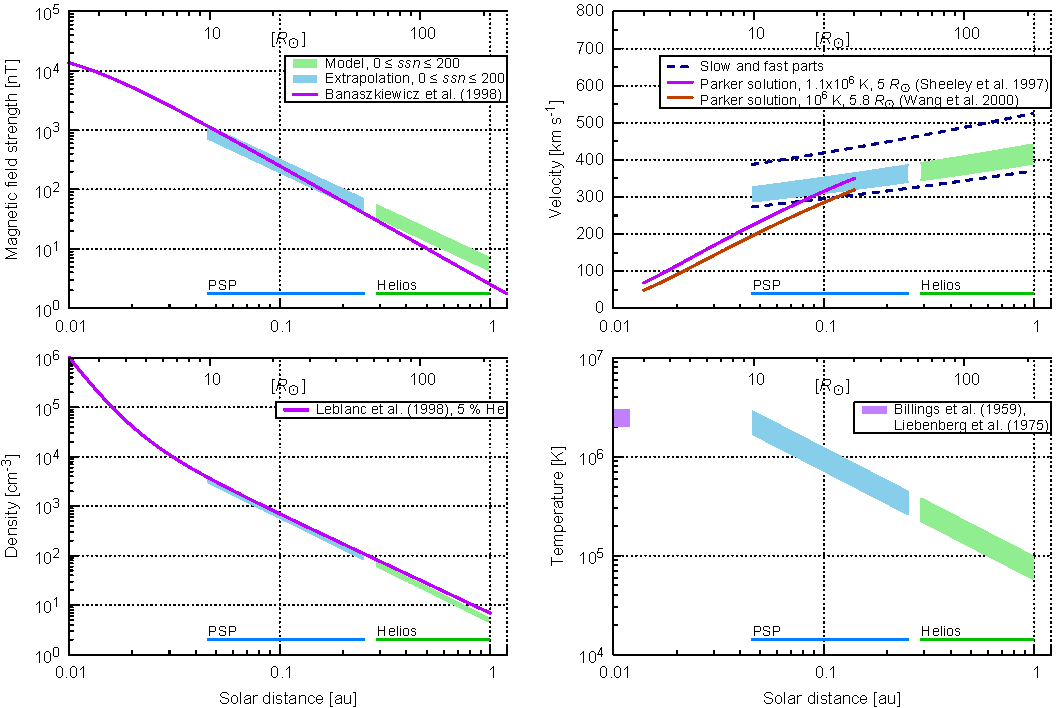
\includegraphics[width=18cm]{figures/sw_extrapolation_ssn_f_plot.pdf}
	\caption{Radial extrapolation of the solar wind parameters to the PSP orbit region. \textbf{The median values from the models, obtained from Helios and OMNI measurements,} are extrapolated to the PSP region \textbf{for SSN values between} solar minimum and maximum, i.e., $0 \le ssn \le 200$\textbf{. The lower edges of the shaded areas correspond to solar minimum, the upper edges to solar maximum.} Also plotted are the radial dependencies of the analytic DQCS magnetic field model for solar minimum from \citet{Banaszkiewicz1998}, the slow wind velocity models from \textbf{\citet{Sheeley1997} and \citet{Wang2000}}, the density model from \citet{Leblanc1998} and the range of temperature measurements from \citet{Billings1959} and \citet{Liebenberg1975}.}
	\label{fig:sw_extrapolation_ssn_f_plot}
\end{figure*}
\textbf{The model and its extrapolation are visualized for the SSN range between solar minimum and maximum ($0 \le ssn \le 200$), indicated by the shaded regions in the figure.}
%magnetic field:
The magnetic field strength is found to increase from median values of about \SI{43}{\nT} at \SI{0.25}{\au} to \SI{715}{\nT} at \SI{0.046}{\au} for a SSN of 0. Taking a SSN of 200 increases the values to \SI{69}{\nT} and \SI{1152}{\nT}. Our extrapolation results are slightly flatter than those derived from the analytical magnetic field model by \citet{Banaszkiewicz1998}, who constructed an analytic dipole plus quadrupole plus current sheet (DQCS) model for solar minimum. \textbf{We note that one cannot straightforeward compare the absolute values of our study with the values obtained by \citet{Banaszkiewicz1998} because the DQCS model assumes solar wind originating from coronal holes at higher heliographic latitudes only, neglecting the slow solar wind belt.}
%Since we cannot compare with their absolute values, because their DQCS model assumes fields of \SI{3.1}{\nT} at \SI{1}{\au} assumed to originate from coronal holes with boundaries at \SI{+-60}{\degree} latitude, excluding the fields from the equatorial slow wind belt.
\textbf{We suggest that the difference in slope is} due to the previously mentioned (Sect.~\ref{sec:solar_distance_dependency}) \textbf{changing shape of the frequency distribution with heliocentric distance}, which for smaller distances deviates more from the model’s lognormal distribution.
%velocity:
The average velocity is found to decrease from \SI{340}{\km\per\s} at \SI{0.25}{\au} to about \SI{290}{\km\per\s} at \SI{0.046}{\au} \textbf{3~years after a} SSN of 0 \textbf{occurred, whereas} using a SSN of 200 it decreases from \SI{390}{\km\per\s} to \SI{330}{\km\per\s}. Comparing the results with the measurements by \citet{Sheeley1997} and \citet{Wang2000} shows an overestimation in our extrapolated slow solar wind velocity values for distances below about \SI{20}{\Rs}. They used LASCO coronagraph observations to track moving coronal features (blobs) in the distance range \SIrange{2}{30}{\Rs} to determine speed profiles and sources of the slow solar wind and they derived temperature and sonic point values for slow solar wind with the isothermal expansion model from \citet{Parker1958}. Therefore, it generally can be expected that PSP will encounter a slower solar wind environment close to the Sun than our model estimates\textbf{. Thus} PSP will measure solar wind acceleration processes \citep{McComas2008}, maybe even still at \SI{30}{\Rs} as the study by \citet{Sheeley1997} suggests.
%density:
The proton density increases from about \SI{84}{\per\cm\cubed} at \SI{0.25}{\au} to about \SI{3018}{\per\cm\cubed} at \SI{0.046}{\au} \textbf{6~years after a SSN of 0 occurred}. Being almost independent of the SSN the values for a SSN of 200 are only \SI{17}{\%} larger. The results are in good agreement with those of \citet{Leblanc1998}, who derived an electron density model from type~III radio burst observations. Their model shows that the density distance dependency scales with $r^{-2}$ and steepens just below \SI{10}{\Rs} with $r^{-6}$. \textbf{We assumed a solar wind helium abundance of \SI{5}{\%} to convert these electron densities to proton densities.}
%temperature:
The extrapolated proton temperature increases from about \SI{260000}{\K} at \SI{0.25}{\au} to about \SI{1690000}{\K} at \SI{0.046}{\au} \textbf{3~years after a SSN of 0 occurred} and from \SI{440000}{\K} to \SI{2860000}{\K} for a SSN of 200. Knowing that near-Sun coronal temperatures are in the range of \SIrange{2}{3}{\mega\K} \citep{Billings1959,Liebenberg1975}, the model \textbf{overestimates} the extrapolated temperatures at the PSP perihelion distance.

%\subsection{SSN prediction for PSP mission time}
%SSN prediction
\textbf{Aside from the solar distance the derived solar wind parameter models depend on the SSN. Short-term predictions of the SSN can be used for the solar wind predictions of PSP's early perihelia and also for refining the solar wind predictions during PSP's mission.} Several sources are available for SSN short-term predictions. The SIDC provides 12-month SSN forecasts\footnote{\url{http://sidc.be/silso/forecasts}} obtained from different methods (e.g., Kalman filter \textbf{Standard Curve} method). The SSN prediction of NOAA's Space Weather Prediction Center (SWPC) follows for the time period until end of 2019 a consensus of the Solar~Cycle~24 Prediction~Panel\footnote{\url{http://www.swpc.noaa.gov/products/solar-cycle-progression}}.
The SSN for PSP's first perihelion will be small -- certainly below 20, whereas \textbf{the SSN during the closest perihelia, which will commence at the end of 2024 at the likely maximum phase of cycle~25, cannot be predicted at this time.} \textbf{However \citet{Hathaway2016} found indications that the next solar cycle will be similar in size to the current cycle~24. Therefore we simply assume a pattern similar to the last cycle for the prediction of the next solar} cycle and thus shift the last cycle by 11~years. Additionally we consider as possible alternatives SSN patterns of half and twice its amplitude as shown in \textbf{the bottom panel of Fig.~\ref{fig:SPP_orbit_predicted_SSN_overview_f_plot}.}

%\subsection{PSP solar wind environment estimation}
Implementing the \textbf{SSN predictions} for the PSP mission time and the orbital trajectory data, \textbf{we can infer} which solar wind parameter magnitudes can be expected. Figs.~\ref{fig:SPP_perihelia_prediction_f_plot} and \ref{fig:SPP_perihelia_prediction_nearest_f_plot} show \textbf{the median values (\ref{eq:median_with_ssn}) of} the considered different solar wind parameters for 12-day periods, comprising the first perihelion in Novemver 2018 and the \textbf{first} closest perihelion in December 2024.
\begin{figure}
	\resizebox{\hsize}{!}{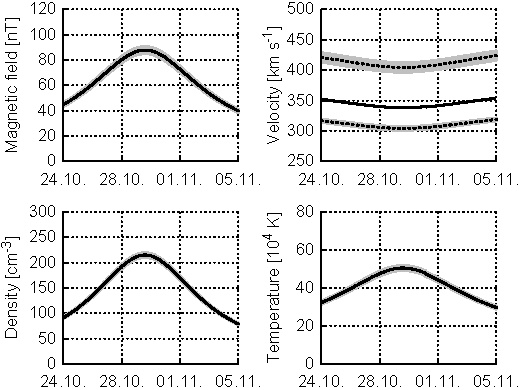
\includegraphics{figures/SPP_perihelia_prediction_f_plot.pdf}}
	\caption{Estimated solar wind parameter medians (black lines) and their error bands (grey) during 12~days in 2018 with PSP's first perihelion at about \SI{0.16}{\au}. For the velocity the combined median is calculated and also the SSN-independent slow and fast parts are plotted (dotted lines).}
	\label{fig:SPP_perihelia_prediction_f_plot}
\end{figure}
% SSN sources and error ranges for first perihelion
% magnetic field:
% SWPC prediction - 0 years
% SWPC expected SSN ranges
% velocity:
% actual monthly SSN - 3 years
% not plotted
% density:
% actual monthly SSN - 6 years
% SIDC given std. dev. from stations
% temperature:
% actual monthly SSN - 3 years
% SIDC given std. dev. from stations
\begin{figure}
	\resizebox{\hsize}{!}{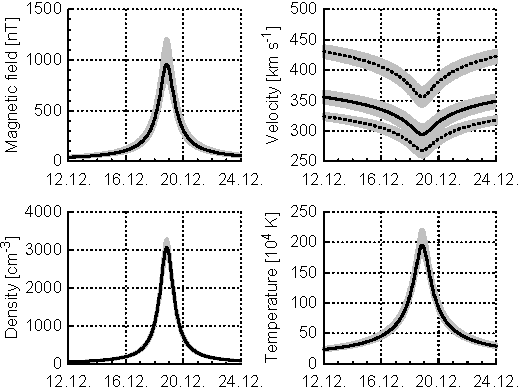
\includegraphics{figures/SPP_perihelia_prediction_nearest_f_plot.pdf}}
	\caption{Estimated solar wind parameter medians (black lines) and their error bands (grey) \textbf{during} 12~days in 2024 with PSP's \textbf{22nd (the first closest)} perihelion at \SI{0.0459}{\au}. For the velocity the combined median is calculated and also the SSN-independent slow and fast parts are plotted (dotted lines).}
	\label{fig:SPP_perihelia_prediction_nearest_f_plot}
\end{figure}
% SSN sources and error ranges for first closest perihelion
% magnetic field:
% actual monthly SSN - 11 years
% half/twice SSN
% velocity:
% actual monthly SSN - 14 years
% not plotted
% density:
% SWPC prediction - 0 years
% SWPC expected SSN ranges
% temperature:
% actual monthly SSN - 14 years
% half/twice SSN
In the beginning of the mission median values of about \SI{87}{\nT}, \SI{340}{\km\per\s}, \SI{214}{\per\cm\cubed} and \SI{503000}{\K} are estimated to be measured at \SI{0.16}{\au}, increasing to about \SI{943}{\nT}, \SI{290}{\km\per\s}, \SI{2951}{\per\cm\cubed} and \SI{1930000}{\K} during the \textbf{first} closest approach at \SI{0.046}{\au}. \textbf{Monthly SSNs -- shifted by the time lags specific to the solar wind parameters -- are used in the calculation of the solar wind predictions. These SSNs are either actual smoothed values from the SIDC with their reported standard deviations, short-term predictions from the SWPC with their expected ranges or actual smoothed values from the SIDC shifted by 11~years with half/twice their values as uncertainties. The error bands given in both figures, calculated from error propagation, include these SSN ranges and the derived fit parameter errors.}
%B
% 87.3642361846083
%N
% 213.613795298952	first
% 2950.67837375615	nearest
% 2925.63248639046	SSN 0
% 3421.59065204775	SSN 200
%T
% 503136.759398494

\textbf{Finally the estimated solar wind environment can be derived from the function $W'''(x,ssn,r)$. The estimated frequency distributions of the four solar wind parameters at PSP's first and 22nd (first closest) perihelion are plotted in Fig.~\ref{fig:SPP_sw_distributions_b}.}
\begin{figure}
	\resizebox{\hsize}{!}{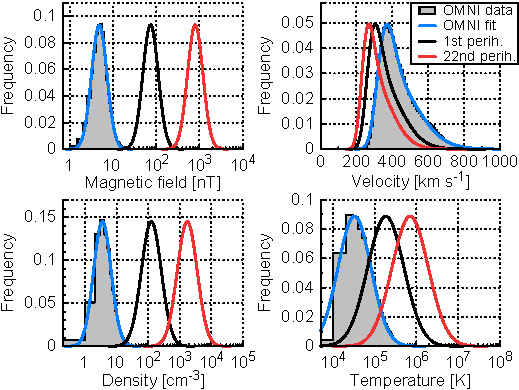
\includegraphics{figures/SPP_sw_distributions_b.pdf}}
	\caption{\textbf{Frequency distributions of the four solar wind parameters (same as in Figs.~\ref{fig:histogram_fits_4_a_zoom_paper_pdfplot} and \ref{fig:histogram_fits_V_a_zoom_dbl_paper_pdfplot}) and those estimated with the solar wind model for PSP's first and 22nd (first closest) perihelion. In these figures the frequencies of both extrapolated curves are scaled for visibility to the same height as the \SI{1}{\au} distribution.}}
	\label{fig:SPP_sw_distributions_b}
\end{figure}
\textbf{Again, we point out that the velocity and temperature distributions for the 22nd perihelion are only upper limits and the actual values to be encountered by PSP are expected to be smaller.}


\section{Discussion and summary}
\label{sec:discussion_and_summary}
\textbf{The scientific objective of this study, being part of the CGAUSS project -- the German contribution to the WISPR instrument, is to model the solar wind environment for the PSP mission to be launched mid 2018. For this purpose we} started the development of the empirical solar wind environment model for the near-ecliptic PSP orbit\textbf{. We derived lognormal representations of the} in situ near-Earth solar wind data collected in the OMNI database, using the frequency distributions of the key solar wind parameters magnetic field strength, \textbf{proton} velocity, density and temperature. Throughout the different analyses in our study the velocity's frequency distribution is treated as a composition of a slow and a fast wind distribution. Each velocity part is fitted with a lognormal function, which allows for the overlap of both velocity ranges. The OMNI multi-spacecraft solar wind data is intercalibrated and covers almost five solar cycles. It thus represents solar wind gathered at different phases of solar activity in the ecliptic plane. In the next step we investigated the yearly variation of the solar wind distribution functions along with the SSN over 53~years and derived linear dependencies of the solar wind parameters with the SSN. The radial dependencies of the solar wind distribution functions were then analyzed, using Helios~1 and 2 data for the distance range \SIrange{0.29}{0.98}{\au} in bins of \SI{0.01}{\au}\textbf{, deriving power law fit functions that} were used to scale the prior calculated SSN-dependent \SI{1}{\au} distribution fit functions to the PSP orbit, \textbf{taking into account} SSN predictions for the years 2018--2025, \textbf{encompassing the prime mission up to the closest approach of \SI{9.86}{\Rs}.} The reason for performing the analysis this way is based on the fact that the OMNI solar wind database is much larger than the Helios database.

\textbf{For determining solar activity and solar distance dependent relations for the median and mean solar wind values, we could have used the simpler approach of combining the radial dependence of averaged Helios data with averaged \SI{1}{\au} OMNI data scaled with the SSN. It is expected that the results of a simpler analysis would have similar distance scaling results, as can be inferred from the exponents in Tables~\ref{tab:mean_median_fit_parameter} and \ref{tab:extrapolation_model_fit_parameters}. However, in our study we are not only interested in averages but rather in bulk distributions, that is, the whole range of values that might occur. For the determination of the frequency distributions the use of the more complex fit model is important, because the distance between median and mean values determines the width of the lognormal distributions.}

\textbf{It} is clear that the calculated distribution functions just represent first order estimates of the real solar wind to be encountered by PSP. The solar wind environment to be encountered will depend at times of PSP on the structure of the solar corona and underlying photospheric magnetic field and on the evolution and interaction of individual solar wind streams and superimposed CMEs and shocks. However, the derived results are in good agreement with existing studies about near-Sun solar wind magnetic field strenghts and densities as shown in Sect.~\ref{sec:model_extrapolation_to_psp_orbit}. \textbf{The extrapolation results of the velocity and the temperature differ from the direct measurements seen in existing studies. This suggests that below about \SI{20}{\Rs} PSP may dive into the region where the acceleration and heating of the solar wind is expected to occur} (see Fig.~\ref{fig:sw_extrapolation_ssn_f_plot}). The near-Sun solar wind velocity at PSP perihelion is also expected to be slower than our model estimates, because the \textbf{solar wind is assumed to be accelerated up to the height of the Alfvénic critical surface, which is predicted to lie on average around \SI{17}{\Rs} \citep[e.g.,][]{Sittler1999,Exarhos2000}, scaling with solar activity within a range of between \SI{15}{\Rs} at solar minimum and \SI{30}{\Rs} at solar} maximum \citep{Katsikas2010,Goelzer2014}.	% in average around 17~Rs (e.g., 0.6~Rs Schatten 1969, 17~Rs Sittler1999, 17~Rs Exarhos2000) and scales with solar activity between 15~Rs in minimum and 30~Rs in maximum (19~Rs Katsikas2010, 15–30~Rs Goelzer2014).

We have not specifically investigated the occurrences of extreme solar wind parameters caused by CMEs or enhanced values due to stream interaction or co-rotating interaction regions. The Helios solar wind measurements plotted over radial distance in Fig.~\ref{fig:radial_fit_4_thesis_light_b_skip} show several extreme values far above the usual solar wind velocities, \textbf{which are} associated with individual CMEs. The results by \citet{Sachdeva2017} indicate that due to \textbf{solar wind drag,} the speeds of fast CMEs will commonly slow down substantially from early distances of a few solar radii. Therefore, it is expected that PSP will encounter CMEs with much higher speeds than those observed during the Helios mission. Also, the magnetic field, density and temperature values are expected to be much larger than in the average solar wind in individual fast shock associated CME events. PSP will thus also substantially improve our understanding of the near-Sun evolution of CMEs and their expansion with radial distance.

%derive heliocentric distance depending error...\\
%error estimation for general model and extreme value tendencies\\

%magnetic field distribution's with distance increasing high value tail -> source are compression regions (why with density no increase?); look into Parker1958's B-field formula...\\
%varying shape with distance is indicator for internal physical processes (mixing/turbulence...)\\

%slow/fast streams basically maintain characteristic speeds with solar cycle; slow/fast ratio SSN dependency\\
%for the overlapping velocity model the SSN dependency is steeper than for a simple threshold\\
%The ratio of both varies with solar activity, e.g., 3~years after maximum, polar coronal holes are observed to often have equatorial extensions (cite?). see and use citet{Bougeret1984} p.~498...\\

%\section{Summary}
%\label{sec:summary}
With the resulting CGAUSS empirical solar wind model for PSP the following main results for the bulk solar wind parameters and estimations for their median values at PSP’s first perihelion in 2018 at a solar distance of \SI{0.16}{\au} and at PSP’s closest perihelia beginning in 2024 at \SI{0.046}{\au} (\SI{9.86}{\Rs}) are obtained:
\begin{itemize}
	\item The dependency of the magnetic field strength \textbf{on solar activity and radial distance appears to be} valid above \SI{20}{\Rs}, however near PSP's closest perihelia the actual values might be found to be slightly higher.
	\item The estimated magnetic field strength \textbf{median values (\ref{eq:median_B})} for PSP's first and \textbf{first} closest perihelion are \SI{87}{\nT} and \SI{943}{\nT}.
	\item The radial dependencies of the proton velocity median values for slow and fast solar \textbf{wind (\ref{eq:median_v}) appear to be} valid above about \SI{20}{\Rs} solar distance, below they overestimate the actual solar wind velocities obtained from remote measurements. The share of their frequency distributions to the overall solar wind velocity distribution (\ref{eq:double_lognormal_fit_function}) is depending on solar activity \textbf{with their balance relation (\ref{eq:balance_v})}. Thus, at solar minimum with \textbf{a SSN} around 0 the slow wind \textbf{component} contributes about \SI{64}{\%} and \textbf{drops} to \SI{28}{\%} during solar maximum conditions with \textbf{a SSN} around 200.
	\item The calculated median velocity values for PSP's first and \textbf{first} closest perihelion are \SI{340}{\km\per\s} and \SI{290}{\km\per\s}.
	\item The \textbf{proton density relation appears to be} valid throughout the full PSP orbital distance range, even down to about \SI{8}{\Rs}.
	\item The estimated density \textbf{median values (\ref{eq:median_n})} for PSP's first and \textbf{first} closest perihelion are \SI{214}{\per\cm\cubed} and \SI{2951}{\per\cm\cubed}.
	\item The derived correlation function for the \textbf{proton temperature appears} to provide too high temperature values \textbf{around PSP’s closest perihelion} in comparison to coronal measurements.
	\item The estimated temperature \textbf{median values (\ref{eq:median_T})} for PSP's first and \textbf{first} closest perihelion are \SI{503000}{\K} and \SI{1930000}{\K}.
\end{itemize}

%Implications for WISPR mission operations and SoloHI on Solar Orbiter...
The results of the modeled solar wind environment will be useful to help optimize the WISPR and in situ instrument science plannings and PSP mission operations. This also applies for the Heliospheric Imager (SoloHI) \citep{Howard2013} and the in situ instruments on board the Solar Orbiter spacecraft.

